\section{Durchführung}
\label{sec:Durchführung}
Für die Durchführung werden zwei verschiedene Apparaturen verwendet, jeweils für Drücke
über bzw. unter $\SI{1}{\bar}$.
\\
Für den Druckbereich $p \leq \SI{1}{\bar}$ kann eine Messapparatur wie in
\autoref{fig:messapparatur1} dargestellt verwendet werden.
\begin{figure}
	\centering
	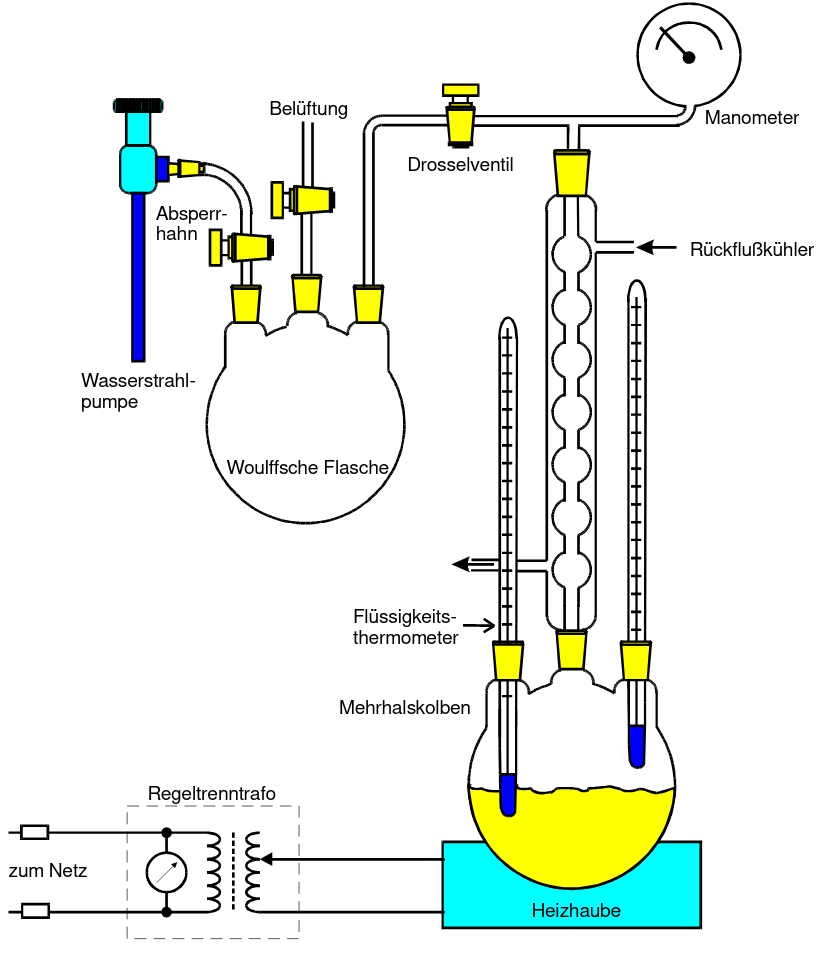
\includegraphics[width=12cm]{images/messapparatur1.png}
	\caption{Skizze der für den Druckbereich $p \leq \SI{1}{\bar}$ verwendeten Messapparatur \cite{anleitung}}
	\label{fig:messapparatur1}
\end{figure}
Zu Beginn muss diese mit einer Wasserstrahlpumpe evakuiert werden, dabei müssen
Absperrhahn und Drosselventil offen und das Belüftungsventil geschlossen sein. Danach kann
mit der Heizhaube das Wasser im Mehrhalskolben erhitzt werden, wobei zeitgleich das
Kühlwasser angeschaltet werden sollte. Das verhindert, dass Dampf in das Manometer
gelangt. Nach Einschalten der Heizung fängt das Wasser an zu sieden und der Druck in der Apparatur
steigt an. Hier sollen die Wasser- und Dampftemperatur sowie der Druck für alle
$\SI{5}{\bar}$ am Flüssigkeitstermometer notiert werden.
\\
Für den Druckbereich $p > \SI{1}{\bar}$ wird die in \autoref{fig:messapparatur2}
skizzierte Apparatur verwendet. Die Probe befindet sich nun in einem Stahlhohlbolzen. Über
ein U-Rohr ist dieser mit einem Drucksensor verbunden. Vor der Messung wird der
Metallkolben mit Wasser gefüllt und gut verschlossen. Danach wird mit einer Heizwicklung
der Bolzen erwärmt und am Drucksensor der Druck abgelesen. Für die Druckwerte $1,2,
\hdots, 15 \si{\bar}$ werden Druck und Temperatur notiert.
\begin{figure}
	\centering
	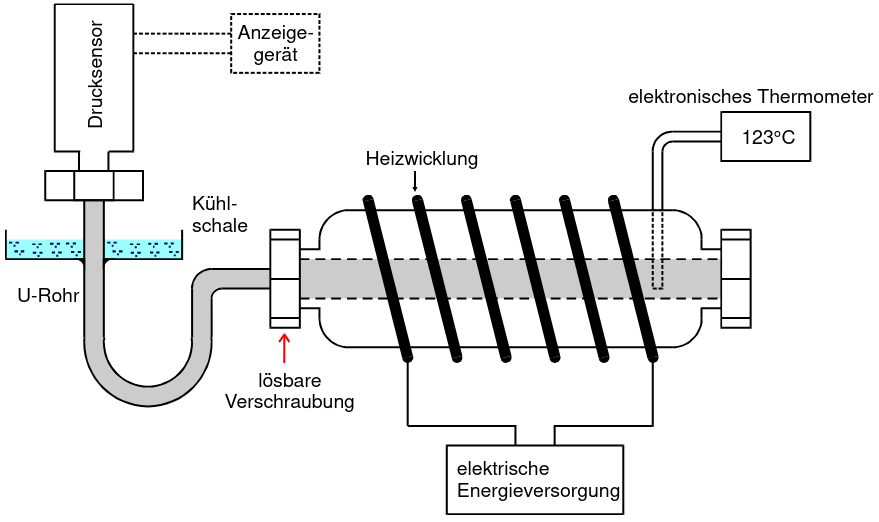
\includegraphics[width=12cm]{images/messapparatur2.png}
	\caption{Skizze der für den Druckbereich $p > \SI{1}{\bar}$ verwendeten Messapparatur \cite{anleitung}}
	\label{fig:messapparatur2}
\end{figure}
